\documentclass{beamer}
\usetheme{metropolis}
\usepackage{../../../resources/style}
\usepackage{colortbl}

\newcommand{\beginnote}[1]{%
  \vfill
  {\footnotesize\textcolor{gray}{\textit{$\triangleright$ #1 (vezi slide-ul \emph{Resurse})}}}%
}

\title{Tipuri de date non-omogene}
\subtitle{Tipul struct $\cdot$ Structuri de date din STL}
\author{Andrei Mihai Ciobanu}
\institute{Algolymp Summer School}
\date{}
\titlegraphic{
\includegraphics[width=4cm]{../../../resources/algolymp-logo.png}}
\setbeamertemplate{frame footer}{Algolymp Summer School}
\setbeamercolor{alerted text}{fg=red!70!black}

\begin{document}

\begin{frame}[shrink]
  \titlepage
\end{frame}

\begin{frame}{Cuprins}
  \tableofcontents
\end{frame}

% ================================================================
\section{Tipul struct}

\begin{frame}[shrink]{Problema: tablouri paralele}
  \begin{center}
  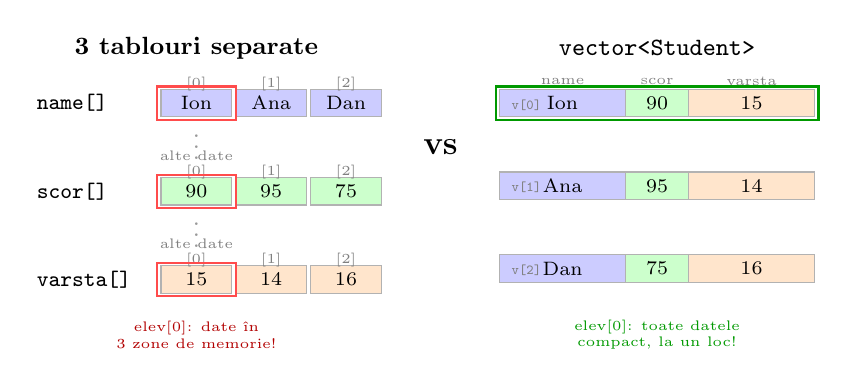
\begin{tikzpicture}[x=1.0cm, y=0.70cm]
    % ZONA 1 (x=0..4.5): 3 tablouri separate
    % ZONA 2 (x=4.5..6.0): separator "vs"
    % ZONA 3 (x=6.0..10.0): vector<Student>  -- fara etichete atarnate spre stanga

    % ===== ZONA 1: 3 tablouri separate =====
    \node[font=\small\bfseries] at (2.15, 8.5) {3 tablouri separate};

    % name[] — celule la x=1.7..4.5, centrate la 2.15 / 3.1 / 4.05
    \node[font=\footnotesize, anchor=west] at (0, 7.5) {\texttt{name[]}};
    \foreach \idx/\na in {0/Ion, 1/Ana, 2/Dan} {
      \fill[blue!20]       (\idx*0.95+1.7, 7.25) rectangle (\idx*0.95+2.6, 7.75);
      \draw[gray!60, thin] (\idx*0.95+1.7, 7.25) rectangle (\idx*0.95+2.6, 7.75);
      \node[font=\tiny, gray]    at (\idx*0.95+2.15, 7.85) {[\idx]};
      \node[font=\scriptsize]    at (\idx*0.95+2.15, 7.5)  {\na};
    }
    \node[font=\small, gray!80] at (2.15, 6.85) {$\vdots$};
    \node[font=\tiny,  gray]    at (2.15, 6.55) {alte date};

    % scor[]
    \node[font=\footnotesize, anchor=west] at (0, 5.9) {\texttt{scor[]}};
    \foreach \idx/\sval in {0/90, 1/95, 2/75} {
      \fill[green!20]      (\idx*0.95+1.7, 5.65) rectangle (\idx*0.95+2.6, 6.15);
      \draw[gray!60, thin] (\idx*0.95+1.7, 5.65) rectangle (\idx*0.95+2.6, 6.15);
      \node[font=\tiny, gray]    at (\idx*0.95+2.15, 6.25) {[\idx]};
      \node[font=\scriptsize]    at (\idx*0.95+2.15, 5.9)  {\sval};
    }
    \node[font=\small, gray!80] at (2.15, 5.25) {$\vdots$};
    \node[font=\tiny,  gray]    at (2.15, 4.95) {alte date};

    % varsta[]
    \node[font=\footnotesize, anchor=west] at (0, 4.3) {\texttt{varsta[]}};
    \foreach \idx/\va in {0/15, 1/14, 2/16} {
      \fill[orange!20]     (\idx*0.95+1.7, 4.05) rectangle (\idx*0.95+2.6, 4.55);
      \draw[gray!60, thin] (\idx*0.95+1.7, 4.05) rectangle (\idx*0.95+2.6, 4.55);
      \node[font=\tiny, gray]    at (\idx*0.95+2.15, 4.65) {[\idx]};
      \node[font=\scriptsize]    at (\idx*0.95+2.15, 4.3)  {\va};
    }

    % Cutii roșii în jurul elementului [0]
    \draw[red!70, thick] (1.65, 7.2) rectangle (2.65, 7.8);
    \draw[red!70, thick] (1.65, 5.6) rectangle (2.65, 6.2);
    \draw[red!70, thick] (1.65, 4.0) rectangle (2.65, 4.6);

    \node[font=\tiny, red!70!black, align=center] at (2.15, 3.3)
      {elev[0]: date în\\3 zone de memorie!};

    % ===== ZONA 2 (x=4.5..6.0): separator =====
    \node[font=\large\bfseries] at (5.25, 6.7) {vs};

    % ===== ZONA 3 (x=6.0..10.0): vector<Student> =====
    % Etichetele v[i] sunt ÎNĂUNTRUL celulelor — nu atârnă spre stânga
    \node[font=\small\bfseries] at (8.0, 8.5) {\texttt{vector<Student>}};

    % Anteturi coloane
    \node[font=\tiny, gray] at (6.8, 7.9) {name};
    \node[font=\tiny, gray] at (8.0, 7.9) {scor};
    \node[font=\tiny, gray] at (9.2, 7.9) {varsta};

    % Rânduri struct
    \foreach \idx/\na/\sval/\va in {0/Ion/90/15, 1/Ana/95/14, 2/Dan/75/16} {
      \fill[blue!20]   (6.0, {7.25-\idx*1.5}) rectangle (7.6, {7.75-\idx*1.5});
      \fill[green!20]  (7.6, {7.25-\idx*1.5}) rectangle (8.4, {7.75-\idx*1.5});
      \fill[orange!20] (8.4, {7.25-\idx*1.5}) rectangle (10.0, {7.75-\idx*1.5});
      \draw[gray!60, thin] (6.0, {7.25-\idx*1.5}) rectangle (10.0, {7.75-\idx*1.5});
      \draw[gray!60, thin] (7.6, {7.25-\idx*1.5}) -- (7.6, {7.75-\idx*1.5});
      \draw[gray!60, thin] (8.4, {7.25-\idx*1.5}) -- (8.4, {7.75-\idx*1.5});
      % v[idx] în colțul stânga-sus al celulei name (înăuntru)
      \node[font=\tiny, gray, anchor=north west]
            at (6.03, {7.74-\idx*1.5}) {\texttt{v[\idx]}};
      \node[font=\scriptsize] at (6.8, {7.5-\idx*1.5}) {\na};
      \node[font=\scriptsize] at (8.0, {7.5-\idx*1.5}) {\sval};
      \node[font=\scriptsize] at (9.2, {7.5-\idx*1.5}) {\va};
    }

    % Cutie verde în jurul v[0]
    \draw[green!60!black, thick] (5.95, 7.2) rectangle (10.05, 7.8);

    \node[font=\tiny, green!60!black, align=center] at (8.0, 3.3)
      {elev[0]: toate datele\\compact, la un loc!};

  \end{tikzpicture}
  \end{center}

  \begin{alertblock}{De ce struct?}
    Un singur \texttt{sort} sau \texttt{swap} mută \textbf{toate câmpurile}
    în bloc \textemdash{} nicio desincronizare posibilă.
  \end{alertblock}
\end{frame}

\begin{frame}[fragile]{Ce este un struct?}
  Multe probleme descriu \textbf{obiecte} cu mai multe proprietăți: \\[6pt]
  \hspace{1cm} produs $=$ \emph{greutate} $+$ \emph{preț} \\
  \hspace{1cm} student $=$ \emph{nume} $+$ \emph{scor} $+$ \emph{vârstă} \\
  \hspace{1cm} eveniment $=$ \emph{timp} $+$ \emph{tip} $+$ \emph{id}

  \smallskip
  Un \textbf{struct} definește un \textbf{tip nou} grupând mai multe câmpuri:

  \begin{lstlisting}
struct produs {
    int greutate;
    double pret;
};
  \end{lstlisting}

  \begin{block}{De reținut}
    \begin{itemize}\itemsep2pt
      \item \texttt{produs} devine un tip la fel ca \texttt{int} sau \texttt{string}
      \item Câmpurile pot fi de \textbf{orice tip}, inclusiv alte struct-uri
    \end{itemize}
  \end{block}
\end{frame}

\begin{frame}[fragile]{Declararea variabilelor struct}
  Odată definit, \texttt{produs} se folosește ca orice alt tip de date:

  \begin{lstlisting}
produs mar;              // o variabila de tip produs
produs banana, pepene;   // mai multe variabile
  \end{lstlisting}

  \smallskip
  Variabilele pot fi declarate și direct în definiție:

  \begin{lstlisting}
struct produs {
    int greutate;
    double pret;
} mar, banana, pepene;
  \end{lstlisting}

  \begin{alertblock}{Struct la nivel global}
    Declară \texttt{struct}-ul \textbf{înainte de \texttt{main()}}.
    Astfel e disponibil în toate funcțiile programului.
  \end{alertblock}
\end{frame}

\begin{frame}[fragile]{Struct \texttt{Student} \textemdash{} exemplu practic}
  Definim un tip \texttt{Student} cu trei câmpuri de tipuri diferite:

  \begin{lstlisting}
struct Student {
    string nume;
    int scor;
    int varsta;
};
  \end{lstlisting}

  \smallskip
  Tipul \texttt{Student} se poate folosi oriunde, ca orice alt tip:

  \begin{lstlisting}
Student elev;           // o singura variabila
Student clasa[30];      // tablou de 30 de studenti
vector<Student> v;      // vector de studenti
  \end{lstlisting}

  \smallskip
  Un struct poate conține câmpuri de \textbf{orice tip}, inclusiv
  \texttt{string}, \texttt{vector}, sau alte struct-uri.
\end{frame}

\begin{frame}[fragile]{Accesul la câmpuri \textemdash{} operatorul \texttt{.}}
  Câmpurile se citesc și se modifică cu \textbf{operatorul punct} (\texttt{.}):

  \begin{lstlisting}
Student s;

// setare campuri
s.nume   = "Ion";
s.scor   = 90;
s.varsta = 15;

// citire campuri
cout << s.nume;        // "Ion"
cout << s.scor + 5;    // 95
cout << s.varsta;      // 15
  \end{lstlisting}

  Fiecare câmp se comportă exact ca o variabilă de tipul său: \\
  \texttt{s.scor} este \texttt{int}, \texttt{s.nume} este \texttt{string}.
\end{frame}

\begin{frame}[fragile]{Inițializare directă cu acolade}
  \begin{lstlisting}
// ordinea campurilor: nume, scor, varsta (ca in struct)
Student s1 = {"Ana", 95, 14};
Student s2 = {"Ion", 90, 15};

// campuri la valoarea implicita (0 pentru numerice, "" pentru string)
Student vid = {};

// mai multe variabile de acelasi tip
Student a, b, c;
a.scor = 10;
b.scor = 20;
c.scor = 30;
  \end{lstlisting}

  \begin{alertblock}{Atenție la ordine}
    \texttt{\{"Ana", 95, 14\}} corespunde câmpurilor în \textbf{exact
    ordinea din definiția struct}.
  \end{alertblock}
\end{frame}

\begin{frame}[fragile]{Tablou de struct-uri}
  Struct-urile se pot pune într-un \textbf{tablou}, ca orice alt tip:

  \begin{lstlisting}
Student cls[30];    // tablou de 30 de studenti
int n;
cin >> n;

for (int i = 0; i < n; i++) {
    cin >> cls[i].nume >> cls[i].scor >> cls[i].varsta;
}

// accesul la campuri: cls[i].camp
cout << cls[0].nume;   // numele primului student
cout << cls[1].scor;   // scorul celui de-al doilea
  \end{lstlisting}

  \begin{block}{Sintaxă}
    \texttt{cls[i].camp} \textemdash{} mai întâi indexul,
    apoi câmpul cu \texttt{.}
  \end{block}
\end{frame}

\begin{frame}[fragile]{Struct în \texttt{vector}}
  Preferăm \texttt{vector<Student>} față de tabloul cu dimensiune fixă:

  \begin{lstlisting}
vector<Student> v;
v.push_back({"Ion", 90, 15});
v.push_back({"Ana", 95, 14});
v.push_back({"Dan", 75, 16});

cout << v[0].nume;    // "Ion"
cout << v[1].scor;    // 95
cout << v.size();     // 3
  \end{lstlisting}

  \begin{block}{Avantaj față de tablouri paralele}
    Un singur \texttt{push\_back} adaugă \textbf{toate câmpurile} simultan.
    Nu mai există risc de desincronizare.
  \end{block}
\end{frame}

\begin{frame}[fragile]{Struct și funcții}
  \begin{lstlisting}
// by reference: eficient, modifica originalul
void mareste_scor(Student& s, int delta) {
    s.scor += delta;
}

// returneaza un struct
Student citeste() {
    Student s;
    cin >> s.nume >> s.scor >> s.varsta;
    return s;
}
  \end{lstlisting}

  \begin{block}{Prin valoare vs.\ prin referință}
    \texttt{void f(Student s)} \textemdash{} copiază struct-ul (costisitor). \\
    \texttt{void f(Student\& s)} \textemdash{} lucrează pe original
    (preferat când vrei să modifici câmpurile).
  \end{block}
\end{frame}

\begin{frame}[fragile]{Sortare cu comparator}
  Vrem: \textbf{scor} $\downarrow$,
  la egalitate \textbf{vârstă} $\uparrow$,
  la egalitate \textbf{nume} lexicografic.

  \begin{lstlisting}
bool cmp(const Student& a, const Student& b) {
    if (a.scor != b.scor)     return a.scor > b.scor;
    if (a.varsta != b.varsta) return a.varsta < b.varsta;
    return a.nume < b.nume;
}

sort(v.begin(), v.end(), cmp);
  \end{lstlisting}

  \begin{alertblock}{Regulă critică}
    Returnează \texttt{false} când elementele sunt egale. \\
    Nu folosi \texttt{<=} sau \texttt{>=}: \texttt{sort} se comportă
    nedefinit (\emph{strict weak ordering}).
  \end{alertblock}
\end{frame}

\begin{frame}{Exemplu}
  \begin{columns}[T]
    \column{0.45\textwidth}
    Date de intrare:
    \begin{center}
    \begin{tabular}{lcc}
      \toprule
      Nume & Scor & Vârstă \\
      \midrule
      ana    & 90  & 15 \\
      bogdan & 90  & 14 \\
      cristi & 100 & 17 \\
      daria  & 90  & 14 \\
      \bottomrule
    \end{tabular}
    \end{center}

    \column{0.52\textwidth}
    \textbf{Rezultat sortat:}
    \begin{enumerate}\itemsep6pt
      \item \textbf{cristi} \textemdash{} scor 100
      \item \textbf{bogdan} \textemdash{} scor 90, vârstă 14
      \item \textbf{daria} \textemdash{} scor 90, vârstă 14,\\
            \texttt{"daria" > "bogdan"}
      \item \textbf{ana} \textemdash{} scor 90, vârstă 15
    \end{enumerate}
  \end{columns}

  \medskip

  Dacă ieșirea este greșită \textbf{doar} la valori egale, bug-ul este
  în comparator.
\end{frame}

% ================================================================
\section{Tipuri de date din STL}

\begin{frame}{Ce este STL?}
  \textbf{STL} (Standard Template Library) face parte din C++ și oferă:

  \begin{itemize}\itemsep6pt
    \item \textbf{Containere} \textemdash{} structuri de date gata de folosit
          (\texttt{vector}, \texttt{set}, \texttt{map}, \ldots)
    \item \textbf{Algoritmi} \textemdash{} \texttt{sort}, \texttt{find},
          \texttt{min\_element}, \ldots
    \item \textbf{Iteratori} \textemdash{} mod de a parcurge containerele, similari cu pointerii
  \end{itemize}

  \smallskip
  \begin{block}{Includere}
    Fiecare container are propriul header: \texttt{\#include <vector>},
    \texttt{\#include <set>}, etc. \\[4pt]
    \texttt{using namespace std;} \textemdash{} necesar pentru toate.
  \end{block}

\end{frame}

\begin{frame}{STL \textemdash{} Categorii de containere}
  STL organizează containerele în \textbf{4 categorii}:

  \smallskip
  \begin{center}
  \footnotesize
  \begin{tabular}{ll}
    \toprule
    Categorie & Containere principale \\
    \midrule
    \textbf{Secvențiale}  & \texttt{vector}, \texttt{deque} \\[3pt]
    \textbf{Adaptoare}    & \texttt{stack}, \texttt{queue}, \texttt{priority\_queue} \\[3pt]
    \textbf{Asociative}   & \texttt{set}, \texttt{multiset}, \texttt{map}, \texttt{multimap} \\[3pt]
    \textbf{Neordonate}   & \texttt{unordered\_set}, \texttt{unordered\_map} \\
    \bottomrule
  \end{tabular}
  \end{center}

  \smallskip
  \begin{block}{Ce să alegi?}
    \begin{itemize}\footnotesize\itemsep1pt
      \item Acces prin index sau sortare? $\rightarrow$ \texttt{vector}
      \item Valori unice sau sortate? $\rightarrow$ \texttt{set}
      \item Asociere cheie/valoare? $\rightarrow$ \texttt{map}
      \item Stivă sau coadă? $\rightarrow$ \texttt{stack} / \texttt{queue}
    \end{itemize}
  \end{block}
\end{frame}

\begin{frame}[fragile]{STL \textemdash{} Algoritmi uzuali}
  Algoritmii STL lucrează pe orice container prin \textbf{iteratori}.
  Incluși în \texttt{<algorithm>}:

  \begin{lstlisting}
#include <algorithm>
vector<int> v = {5, 2, 8, 1, 9, 3};

sort(v.begin(), v.end());              // [1,2,3,5,8,9]
reverse(v.begin(), v.end());           // [9,8,5,3,2,1]

sort(v.begin(), v.end());
int mx = *max_element(v.begin(), v.end()); // 9

// cauta valoarea 5 (vectorul trebuie sortat)
bool ex = binary_search(v.begin(), v.end(), 5); // true
int nr = count(v.begin(), v.end(), 5);           // 1
  \end{lstlisting}

  \smallskip
  Toți algoritmii primesc \textbf{iteratori de început și de final}:
  \texttt{v.begin()} și \texttt{v.end()}.
\end{frame}

\begin{frame}[fragile]{1. vector \textemdash{} operații de bază}
  \texttt{vector<T>} funcționează ca un tablou, dar cu \textbf{lungime variabilă}:

  \begin{lstlisting}
#include <vector>
vector<int> v;

v.push_back(3);    // v = [3]
v.push_back(7);    // v = [3, 7]
v.push_back(1);    // v = [3, 7, 1]

cout << v[0];      // 3   (indexare de la 0)
cout << v.size();  // 3
v.pop_back();      // v = [3, 7]
cout << v.empty(); // 0 (false)
v.clear();         // v = []
  \end{lstlisting}

  \texttt{push\_back}: $O(1)$ în medie. \quad
  \texttt{v[i]}: $O(1)$.
\end{frame}

\begin{frame}[fragile]{1. vector \textemdash{} inițializare și parcurgere}
  \begin{lstlisting}
// initializare cu n elemente = 0
vector<int> a(5, 0);    // [0, 0, 0, 0, 0]

// initializare cu valori
vector<int> b = {3, 1, 4, 1, 5};

// parcurgere cu indice
for (int i = 0; i < (int)b.size(); i++) {
    cout << b[i] << " ";    // 3 1 4 1 5
}
// parcurgere for-each
for (int x : b) {
    cout << x << " ";
}
// sortare
sort(b.begin(), b.end());   // b = [1, 1, 3, 4, 5]
  \end{lstlisting}
\end{frame}

\begin{frame}[fragile]{2. pair \textemdash{} pereche de valori}
  \texttt{pair<T1,\,T2>} stochează două valori accesate cu
  \texttt{.first} și \texttt{.second}:

  \begin{lstlisting}
#include <utility>

pair<int, int> p = {3, 7};
cout << p.first;    // 3
cout << p.second;   // 7

// sortare automata: intai dupa first, la egalitate dupa second
vector<pair<int,int>> v = {{5,2}, {3,8}, {3,1}};
sort(v.begin(), v.end());
// v = [(3,1), (3,8), (5,2)]
  \end{lstlisting}

  \smallskip
  Un \texttt{pair} e ca un struct cu doi câmpi anonimi.
  Util pentru a returna două valori dintr-o funcție sau
  pentru chei compuse în \texttt{map}.
\end{frame}

\begin{frame}[fragile]{3. string \textemdash{} șir de caractere}
  \begin{lstlisting}
#include <string>

string s = "hello";
s.size();           // 5
s[1];               // 'e'
s += " world";      // s = "hello world"

// subsir de la pozitia 6, lungime 5
s.substr(6, 5);     // "world"

// prima aparitie; npos daca nu gaseste
s.find("world");    // 6

// comparare lexicografica cu ==, <, >
"abc" < "abd";      // true
  \end{lstlisting}

  \smallskip
  \texttt{string} se comportă ca un \texttt{vector<char>}:
  are \texttt{push\_back}, \texttt{size}, parcurgere cu \texttt{for}.
\end{frame}

\begin{frame}[fragile]{4. set \textemdash{} elemente unice, sortate}
  \texttt{set<T>}: elemente \textbf{unice}, menținute automat în
  \textbf{ordine crescătoare}. Toate operațiile: $O(\log n)$.

  \begin{lstlisting}
#include <set>
set<int> s;
s.insert(3);     // s = {3}
s.insert(1);     // s = {1, 3}  <- sortat automat
s.insert(3);     // ignorat!    s = {1, 3}

s.count(3);      // 1  (exista)
s.count(7);      // 0  (nu exista)
s.erase(3);      // s = {1}

for (int x : s) cout << x;   // in ordine crescatoare
  \end{lstlisting}
\end{frame}

\begin{frame}[fragile]{4. set \textemdash{} căutare și multiset}
  \begin{lstlisting}
set<int> s = {1, 3, 5, 9, 14};

// cel mai mic element >= k
auto it = s.lower_bound(5);
cout << *it;      // 5
// cel mai mic element > k
auto it2 = s.upper_bound(5);
cout << *it2;     // 9
// cel mai mare element
auto last = s.end(); --last;
cout << *last;    // 14
  \end{lstlisting}

  \begin{block}{multiset \textemdash{} duplicate permise}
    \texttt{multiset<int> ms;} \\
    \texttt{ms.insert(3); ms.insert(3);} $\rightarrow$ \texttt{\{3,\,3\}} \\
    \texttt{ms.count(3)} $= 2$
  \end{block}
\end{frame}

\begin{frame}[fragile]{5. map \textemdash{} cheie $\rightarrow$ valoare}
  \texttt{map<K,\,V>} asociază chei unice cu valori.
  Cheile sunt sortate automat, $O(\log n)$ per operație.

  \begin{lstlisting}
#include <map>
map<string, int> freq;
freq["mere"] = 5;
freq["pere"] = 3;
freq["mere"]++;         // freq["mere"] = 6

cout << freq["mere"];   // 6

// verifica existenta fara a crea cheia
freq.count("prune");    // 0  (nu exista)
if (freq.count("mere"))
    cout << freq["mere"]; // 6

freq.erase("pere");
  \end{lstlisting}
\end{frame}

\begin{frame}[fragile]{5. map \textemdash{} parcurgere și multimap}
  \begin{lstlisting}
map<string, int> freq;
freq["ana"] = 3;
freq["dan"] = 2;
freq["ion"] = 1;

// parcurgere in ordine alfabetica dupa cheie
for (auto& p : freq) {
    cout << p.first << ": " << p.second << "\n";
}
// ana: 3
// dan: 2
// ion: 1
  \end{lstlisting}

  \begin{block}{multimap \textemdash{} chei duplicate}
    Permite mai multe valori pentru aceeași cheie. \\
    Rar folosit: \texttt{map<K,\,vector<V>>} este de obicei mai flexibil.
  \end{block}
\end{frame}

\begin{frame}[fragile]{6. unordered\_set și unordered\_map}
  Variante bazate pe \textbf{hashing}: $O(1)$ în medie, dar \textbf{nesortate}.

  \begin{columns}[T]
    \column{0.48\textwidth}
    \begin{block}{\texttt{set} / \texttt{map}}
      \begin{itemize}\footnotesize\itemsep1pt
        \item Sortat automat
        \item $O(\log n)$ garantat
        \item \texttt{lower\_bound} disponibil
        \item Sigur pe concursuri
      \end{itemize}
    \end{block}

    \column{0.48\textwidth}
    \begin{block}{\texttt{unordered\_*}}
      \begin{itemize}\footnotesize\itemsep1pt
        \item Nesortat
        \item $O(1)$ în medie
        \item Fără \texttt{lower\_bound}
        \item Poate fi atacat cu date special construite
      \end{itemize}
    \end{block}
  \end{columns}

  \smallskip
  \begin{lstlisting}
#include <unordered_set>
#include <unordered_map>
unordered_set<int> us = {3, 1, 4, 1, 5};
unordered_map<string, int> um;
um["a"] = 1;  um["b"] = 2;
  \end{lstlisting}
\end{frame}

\begin{frame}[fragile]{7. stack, queue, deque}
  \begin{columns}[T]
    \column{0.33\textwidth}
    \begin{block}{\texttt{stack} \textemdash{} LIFO}
      \begin{lstlisting}
stack<int> st;
st.push(3);
st.push(7);
st.top();  // 7
st.pop();
st.top();  // 3
      \end{lstlisting}
    \end{block}

    \column{0.33\textwidth}
    \begin{block}{\texttt{queue} \textemdash{} FIFO}
      \begin{lstlisting}
queue<int> q;
q.push(3);
q.push(7);
q.front(); // 3
q.pop();
q.front(); // 7
      \end{lstlisting}
    \end{block}

    \column{0.33\textwidth}
    \begin{block}{\texttt{deque}}
      \begin{lstlisting}
deque<int> d;
d.push_back(3);
d.push_front(1);
// [1, 3]
d.pop_back();
d.pop_front();
      \end{lstlisting}
    \end{block}
  \end{columns}

  \smallskip
  \begin{itemize}\footnotesize\itemsep0pt
    \item \texttt{stack}: ultimul intrat = primul ieșit (stivă)
    \item \texttt{queue}: primul intrat = primul ieșit (coadă)
    \item \texttt{deque}: inserare/ștergere la ambele capete
  \end{itemize}
\end{frame}

\begin{frame}[fragile]{priority\_queue \textemdash{} coadă cu priorități}
  Max-heap implicit: \texttt{top()} returnează întotdeauna \textbf{maximul}.

  \begin{lstlisting}
#include <queue>
priority_queue<int> pq;
pq.push(3);
pq.push(7);
pq.push(1);
cout << pq.top();   // 7  (maximul)
pq.pop();
cout << pq.top();   // 3
  \end{lstlisting}

  \begin{block}{Min-heap}
    \texttt{priority\_queue<int, vector<int>, greater<int>> pq\_min;} \\
    \texttt{pq\_min.top()} returnează \textbf{minimul}.
  \end{block}
\end{frame}

\begin{frame}[fragile]{tuple și bitset}
  \begin{block}{\texttt{tuple} \textemdash{} generalizare a lui \texttt{pair}}
    Poate stoca oricâte valori; accesate cu \texttt{get<i>}:
    \begin{lstlisting}
#include <tuple>
tuple<int, string, double> t = {1, "abc", 3.14};
get<0>(t);   // 1
get<1>(t);   // "abc"
get<2>(t);   // 3.14
    \end{lstlisting}
  \end{block}

  \begin{block}{\texttt{bitset<N>} \textemdash{} secvență fixă de $N$ biți}
    \begin{lstlisting}
#include <bitset>
bitset<8> b("10110101");
b.count();    // 5  (biti de 1)
b.set(0);     // seteaza bitul 0
b[3];         // acces bit
    \end{lstlisting}
  \end{block}
\end{frame}

% ================================================================
\section{Recapitulare}

\begin{frame}{Probleme de antrenament}
  \begin{enumerate}\itemsep8pt
    \item \href{https://cses.fi/problemset/task/1621}{\textbf{Distinct Numbers}}
          \textcolor{gray}{(CSES \#1621)}
    \item \href{https://code.algolymp.com/problems/4278}{\textbf{Student Registry STL}}
          \textcolor{gray}{(AlgoCode \#4278)}
  \end{enumerate}
\end{frame}

\begin{frame}{Resurse}
  \begin{columns}[T]
    \column{0.46\textwidth}
    \textbf{Română}
    \begin{itemize}\footnotesize\itemsep1pt
      \item \href{https://cplusplus.com/doc/tutorial/structures/}{\textbf{cplusplus.com}}
            \textemdash{} tutorial structuri C++
      \item \textbf{pbinfo.ro}:
      \begin{itemize}\tiny\itemsep0pt
        \item \href{https://www.pbinfo.ro/articole/7652/structuri-de-date-neomogene-in-cpp}{Structuri de date neomogene}
        \item \href{https://www.pbinfo.ro/articole/7653/tipul-struct}{Tipul struct}
        \item \href{https://www.pbinfo.ro/articole/7654/operatii-cu-structuri}{Operații cu structuri}
        \item \href{https://www.pbinfo.ro/articole/7655/structuri-imbricate}{Structuri imbricate}
        \item \href{https://www.pbinfo.ro/articole/7656/structuri-tablouri-si-functii}{Structuri, tablouri și funcții}
        \item \href{https://www.pbinfo.ro/articole/23702/standard-template-library-stl}{Standard Template Library (STL)}
      \end{itemize}
    \end{itemize}

    \column{0.54\textwidth}
    \textbf{Engleză}
    \begin{itemize}\footnotesize\itemsep1pt
      \item \href{https://cses.fi/book/book.pdf}{\textbf{CPH}}
            \textemdash{} cap.\ 4: Data Structures
      \item \textbf{GeeksforGeeks}:
      \begin{itemize}\tiny\itemsep0pt
        \item \href{https://www.geeksforgeeks.org/cpp/the-c-standard-template-library-stl/}{STL in C++}
        \item \href{https://www.geeksforgeeks.org/cpp/structures-in-cpp/}{Structures in C++}
      \end{itemize}
      \item \textbf{USACO Guide}:
      \begin{itemize}\tiny\itemsep0pt
        \item \href{https://usaco.guide/bronze/intro-ds}{Intro to Data Structures} (Bronze)
        \item \href{https://usaco.guide/bronze/intro-sets}{Intro to Sets \& Maps} (Bronze)
        \item \href{https://usaco.guide/gold/intro-sorted-sets}{Sorted Sets} (Gold)
        \item \href{https://usaco.guide/gold/custom-cpp-stl}{Custom Comparators} (Gold)
      \end{itemize}
      \item \textbf{Programiz}:
      \begin{itemize}\tiny\itemsep0pt
        \item \href{https://www.programiz.com/cpp-programming/structure}{C++ Structures}
        \item \href{https://www.programiz.com/cpp-programming/structure-function}{Structure \& Function}
      \end{itemize}
    \end{itemize}
  \end{columns}
\end{frame}

\end{document}
